\documentclass[
    parskip=half, 
    twoside=false,
    twocolumn=true,
    fontsize=11pt,
]{scrarticle}
\usepackage{xcolor}
\definecolor{seeblau}{HTML}{00A9E0}
\definecolor{seegrau}{HTML}{9AA0A7}

\definecolor{seeblau1}{HTML}{CCEEF9}
\definecolor{seeblau2}{HTML}{A6E1F4}
\definecolor{seeblau3}{HTML}{59C7EB}
\definecolor{seeblau4}{HTML}{00A9E0}
\definecolor{seeblau5}{HTML}{008ECE}


\usepackage{graphicx}
\usepackage{amsmath}
\usepackage{subcaption}
\usepackage{wrapfig}
\usepackage[english]{babel}
\usepackage{blindtext}
\usepackage{microtype}
\usepackage{siunitx}
\usepackage[utf8]{inputenc}
\usepackage{csquotes}
\usepackage{nicefrac}
\usepackage[T1]{fontenc}
\usepackage{amsfonts}
\usepackage{amssymb}
\usepackage{tikz}

\usepackage{siunitx}

\usepackage{libertinus, libertinust1math}
\usepackage{roboto}

\setkomafont{disposition}{\normalfont\sffamily}


% not recommended with KOMA-script
% make table of contents sans-serif
% \usepackage{tocloft}
% \renewcommand\cftchappagefont{\normalfont}
% \renewcommand\cftchapfont{\normalfont}
% \renewcommand\cftchappresnum{\bfseries}
% \renewcommand\cftchapaftersnum{}
% \renewcommand{\cftchapfont}{\sffamily}
% \renewcommand{\cftsecfont}{\sffamily}
% \renewcommand{\cftsubsecfont}{\sffamily}
% \renewcommand{\cftchappagefont}{\sffamily}
% \renewcommand{\cftsecpagefont}{\sffamily}
% \renewcommand{\cftsubsecpagefont}{\sffamily}

% caption
\usepackage{caption}
\captionsetup{
	% font={sf},
	labelfont={sf, bf, color=seeblau},
	labelsep=quad,
	labelformat=simple,
}

% links
\usepackage{hyperref}
\hypersetup{
	colorlinks=true,
	linkcolor=seeblau,
	citecolor=seeblau,
	urlcolor=seeblau,
	% hidelinks=true
}

% bibliography
\usepackage[
	style=numeric-comp, % comp = compressed 4,5,6,7 -> 4-7
	sorting=none,		% Sort by appearance
	% autocite = superscript,
	% backref=true,
	hyperref=true,
	url=true,
	maxbibnames=100
]{biblatex}
\DefineBibliographyStrings{english}{%
    backrefpage  = {see p.}, % for single page number
    backrefpages = {see pp.} % for multiple page numbers
}

% remove issue
\AtEveryBibitem{%
  \clearfield{number}
}

\usepackage{float}
% \floatplacement{figure}{h}
% \floatplacement{table}{H}

% loosen float placement rules
\renewcommand{\topfraction}{0.8}
\renewcommand{\bottomfraction}{.8}
\renewcommand{\textfraction}{0.1}
\renewcommand{\floatpagefraction}{.9}
% make floats less likely to be placed on a separate page
\setcounter{totalnumber}{9}
\setcounter{topnumber}{9}
\setcounter{bottomnumber}{9}

% decrease space between floats and text
\setlength{\textfloatsep}{0.5cm}
\setlength{\floatsep}{0.5cm}


\usepackage{adjustbox}

\usepackage{datetime}
\newdateformat{dotdate}{
	\twodigit{\THEDAY}.\twodigit{\THEMONTH}.\THEYEAR
}
\newdateformat{monthyeardate}{%
  \monthname[\THEMONTH] \THEYEAR}


% header and footer
\usepackage[
  markcase=noupper
]{scrlayer-scrpage}% activates pagestyle scrheadings automatically
\clearpairofpagestyles
\setkomafont{pageheadfoot}{\normalfont\sffamily}
\setkomafont{pagenumber}{\normalfont\sffamily}
% \chead*{\color{seegrau} Draft \dotdate\today}
\ofoot*{\pagemark}
\ohead*{\rightmark}


\usepackage{ifthen}
\newcommand{\markieren}[4]{
    \ifthenelse{\equal{#1}{}}{}{\adjustbox{padding=3pt, bgcolor=seeblau1, margin=-1pt}{\strut{\sffamily\robotoMedium{#1}}}\\}
    \ifthenelse{\equal{#2}{}}{}{\adjustbox{padding=3pt, bgcolor=seeblau2, margin=-1pt}{\strut{\sffamily\robotoMedium{#2}}}\\}
	\ifthenelse{\equal{#3}{}}{}{\adjustbox{padding=3pt, bgcolor=seeblau3, margin=-1pt}{\strut{\sffamily\robotoMedium{#3}}}\\}
	\ifthenelse{\equal{#4}{}}{}{\adjustbox{padding=3pt, bgcolor=seeblau4, margin=-1pt}{\strut{\sffamily\robotoMedium{#4}}}}
}

\addbibresource{literature.bib}

\begin{document}

\title{title}
\subtitle{subtitle}
\author{Aurel Müller-Schoenau, Leon Oleschko}
\date{\dotdate\today}


% make a custom title page
\begin{titlepage}
    \sffamily
    \vspace*{3cm}
    {
        \fontsize{32}{32}
        \markieren{}{Johnson-Nyquist}{und Schottky}{Rauschen}
    }
    \vspace{.25cm}\\
    {
        \Large
        Aurel Müller-Schoenau, Leon Oleschko\\
        Supervised by Richard Schlitz
        \vspace{.05cm}\\
        27. November 2024
        \vspace{.25cm}\\
        \normalsize
        Physikalisches Fortgeschrittenenpraktikum 2\\
        Universität Konstanz
    }
    \vfill
    {
        \normalfont\normalsize
        We investigate Johnson-Nyquist noise and Shot noise.
        By measuring voltage fluctuations across resistors with varying resistance, bandwidth and temperatures, we determine the Boltzmann constant and estimate the absolute zero temperature. 
        Additionally, we measure the Shot noise of a photodiode, demonstrating the advantage of using a transimpedance ampl ifier to calculate the elementary charge.
        Despite some deviations due to unknown additional noise sources, our results demonstrate the fundamental properties of electrical noise and its application in determining physical constants.
    }
    \vfill
    \begin{flushright}
        Available at \url{www.github.com/leoole100/fp2}.
    \end{flushright}
\end{titlepage}

\section{Introduction}

All measurements conducted in the real world are subject to some form of noise. What is often regarded an obstacle may provide some important information about the system that is being observed. In this experiment, we take a look at two types of noise, namely Johnson-Nyquist noise occuring in an electrical resistor and Shot noise of a photo diode. Some of the properties of these types of noise are universal and will allow us to derive the Boltzmann constant and the elementary charge as well as the point of absolute zero temperature.

\section{Setup}
For this experiment, the setup \textit{Noise Fundamentals NF1-A} by \textit{TeachSpin, Inc.} was used. It consists of a low level electronics (LLE) component with a built-in preamplifier, and in a separate enclosure the High Level Electronics such as an additional output amplifier, frequency filters and a voltage squaring circuit.\\
The resistors used in the first part of the experiment are built directly into the LLE setup, whereas the module carrying the photo diode and lamp to measure shot noise has to be connected separately. An additional probe with resistors sits inside a Dewar which can hold liquid Nitrogen. Since we are measuring wide-band noise, the measurement bandwidth is important. The effective bandwidth resulting from the settings in the HLE component is taken from a table provided in the setup manual \autocite{instructions}.\\
Measurements are taken with a multimeter connected to the output of the HLE. The statistical uncertainty of the voltmeter was measured to be $\sigma = \SI{0.001}{V}$.

\subsection*{Oscilloscope}
A oscilloscope, can alternatively be used to measure the noise and to apply digital filtering after the experiment.
The disadvantages are a larger additional quantisation noise, as the analog digital converters in oscilloscopes have a lower resolution than multimeters.
Additionally the spectral bandwidth is limited by the sampling frequency and the memory depth.\\
An oscilloscope connected to the setup was supposed to be used to digitize the voltage.
To validate the correct function of the instruments, the oscilloscope was set to measure the AC Root Mean Square voltage, calculating it in the digital domain, while the multimeter was set to AC voltage, doing the same in the analog domain.
But, we found that the readings on the oscilloscope differed significantly from what the multimeter was showing, and were susceptible to axis scaling on the oscilloscope graph, that was not consistent with expectations.
The device was ruled out of the experiment due to what we consider a firmware bug.

\section{Johnson-Nyquist Noise}


\begin{figure}
    \centering
    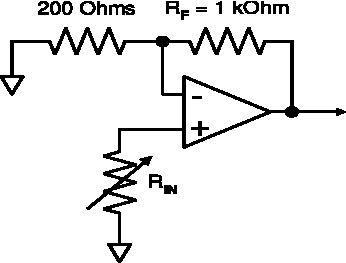
\includegraphics[width=0.4\textwidth]{figures/measure_R_setup_part1.pdf}
    \caption{
        Schematic for the setup to measure Johnson noise across an ohmic resistor $R_\text{IN}$ as provided by \autocite{instructions}.
    }
    \label{fig:johnson setup R}
\end{figure}


Conducting an experiment at room temperature means that a certain amount of thermal excitation is going to be present. The voltage across an electric component such as a simple ohmic resistor therefore shows small fluctuations. This so-called \textit{Johnson-Nyquist Noise} is white noise. Its power spectral density is quantified by the voltage variance

\begin{equation}
    \label{eq:johnson noise}
    S\;\Delta f = \langle V_J^2 \rangle = 4\; k_B T\; R\; \Delta f + S_0\, \Delta f
\end{equation} 

Where $k_B$ is the Boltzmann constant, $T$ is temperature and $R$ is the electric resistance of the resistor. The bandwidth $\Delta f$ is crucial since the data is measured digitally. It is adjusted using the high pass and low pass filters in the HLE component. The offset $S_0$ was added to the equation taken from \autocite{Buch}. It has its roots in the signal processing chain and is assumed to be white noise. 
Using the setup to probe a very small resistance should yield $S_0$, but it can also be eliminated from the equation by taking the derivate with respect to $R$, assuming that resistor and amplifier operate independently.\\
The schematic for this measurement is shown in \autoref{fig:johnson setup R}. The resistor $R_\text{IN}$ is the one being probed. The preamplifier has a gain of $6$.  According to \autoref{eq:johnson noise}, the noise is linear in $R$ and $\Delta f$. It was measured for varying resistors and bandwidths.
\begin{figure*}[h!]
    \centering
    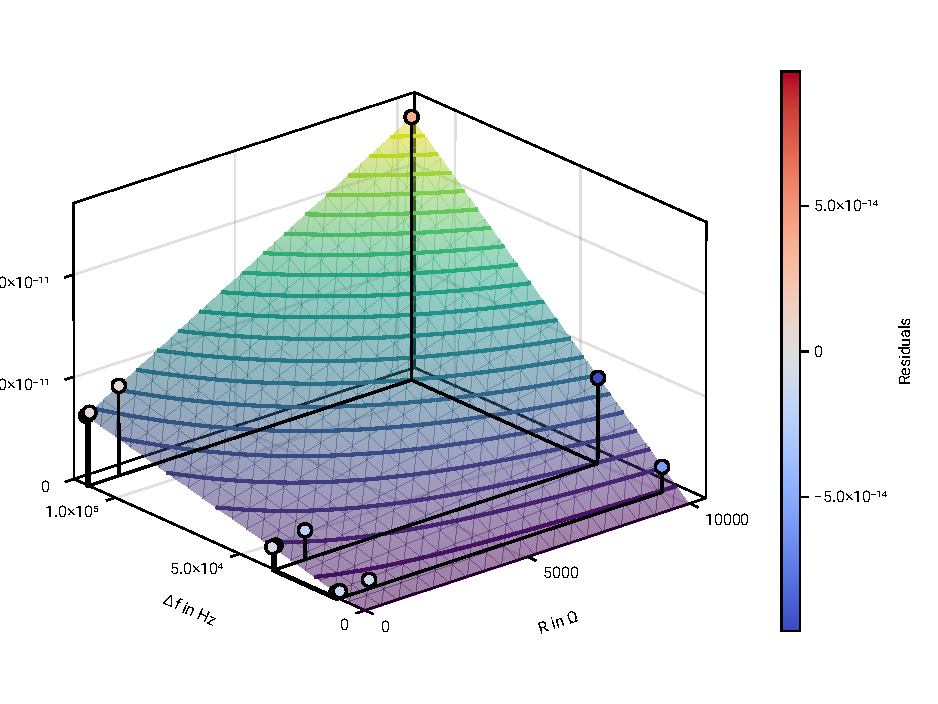
\includegraphics{figures/05 johnson noise rt plane.pdf}
    \caption{
        Measured noise density over different resistors and bandwidths.
        Fit according to \autoref{eq:johnson noise}, fit residuals as colors.
    }
    \label{fig:johnson noise}
\end{figure*}

Our data in \autoref{fig:johnson noise} clearly fits the model \autoref{eq:johnson noise}. 
The fit residuals were very small, owing to the fact that this part of the experiment is hard-wired into the LLE setup, with short wires and consistent electrical connections.
Despite that, the value computed for the Boltzmann constant $k_B = \SI{1.433(1.5)e-23}{J/K}$ differs significantly from the literature value of $\SI{1.380e-23}{J/K}$. 
The uncertainty is calculated from the fit, and $T = \SI{295(3)}{K}$.
The noise of the amplifier can be estimated to be $S_0 = \SI{6.213(15)e-7}{(\mu V)^2/Hz}$.\\
The overestimated $k_B$ implies additional noise sources that correlate with $R$ and $\Delta f$, or with $S$.
\textit{
    One possible explanation is a frequency-dependent component to the preamplifier noise, but this would not explain any change in behaviour for measurements with varying resistance but constant bandwidth.
    Another possibility is noise generated by the second amplifier stage.
    In that case, the noise component added to the signal would vary in magnitude relative to the signal due to variable gain.
    This was not taken into consideration during the experiment.
}

\subsubsection*{Temperature Measurement}
\begin{figure*}[h!]
    \centering
    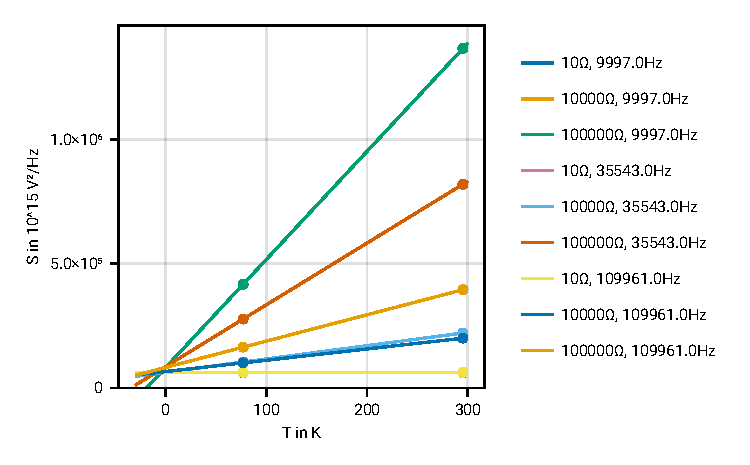
\includegraphics{figures/02 temperature.pdf}
    \caption{
        Measured noise density over temperature for different resistors and bandwidths.
        The measured noise of the amplifier is 
    }
    \label{fig:johnson noise temperature}
\end{figure*}
In the previous section, the absolute room temperature was assumed to be already known. 
However, since \autoref{eq:johnson noise} is linear in $T$ (neglecting the offset noise $S_0$, which has already been quantified) extrapolating the measured data to the point where the noise vanishes should yield the value $T$ at absolute zero. 
To do this, a probe containing several resistors is lowered into a Dewar. 
The probe is connected to the LLE using an otherwise similar setup to \autoref{fig:johnson setup R}. The noise RMS was measured at room temperature (\SI{295(3)}{K}) and with the probe submerged in liquid Nitrogen (\SI{77(3)}{K}). Again, the measurement was conducted for different resistors and bandwidths.

% The measured zero temperature is \SI{-6.4(15)}{K}. The measurement errors were so small that the uncertainty was calculated from only the spread of data points, but the result implies other error sources.
% \textbf{Discuss differing procedure, reasons for the uncertainties and the bandwidth dependency.}

The resulting noise measurements are shown in \autoref{fig:johnson noise temperature} including linear fits.
There are two notable observations: 
Firstly, the smallest resistor (\SI{10}{\ohm}) behaves like a short circuit in that the measured noise does not depend on temperature. 
The majority of it must be coming from another source, which is not very surprising knowing that Johnson noise depends linearly on resistance.\\
Probing a resistor of \SI{10}{\kilo\ohm} yielded the expected result. 
With the spectral noise density $S$ being independent of the bandwidth and proportional to the temperature.\\
But the results from the \SI{100}{\kilo\ohm}-measurement are puzzling: Here, noise actually decreases with increasing bandwidth.
As the same frequency bands were used for the \SI{10}{\kilo\ohm} resistor, where no such effect was observed, the noise source has to depend on resistance. 
For example, there might be an additional noise current which creates a higher voltage across the bigger resistor.
Another complication, however is that the additional noise is also dependent on temperature. 
This should only be the case for Johnson noise, which would behave differently. 
We might be observing a nonlinear effect of an additional noise source which generates more noise the stronger the already existing signal is.
Either way, more measurements would be needed to pin down the source.

\begin{figure}[h!]
    \centering
    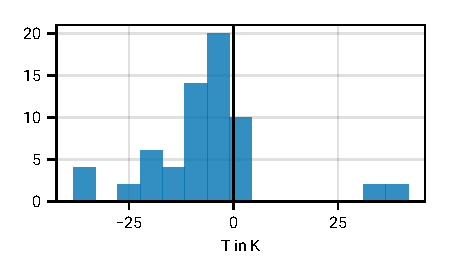
\includegraphics{figures/02 temperature distribution.pdf}
    \caption{
        Distribution of the measured temperature by looking at the crossings of the linear fits in \autoref{fig:johnson noise temperature}.
    }
    \label{fig:johnson noise temperature distribution}
\end{figure}
Because of all that, interpreting the results from this part of the experiment is difficult. 
Computing the point of absolute zero temperature by extrapolating linearly to the axis intersection yields the results shown in \autoref{fig:johnson noise temperature distribution}. Most of them lie significantly below \SI{0}{\kelvin}. The mean result is \SI{-6.4(15)}{\kelvin}.
This result can be improved by making arbitrary assumptions about the additional noise, but this approach is vague without a proper model for the additional noise.
\textbf{Make such a assumption to calculate a value.}

\section{Shot Noise}
\begin{figure}[h!]
    \centering
    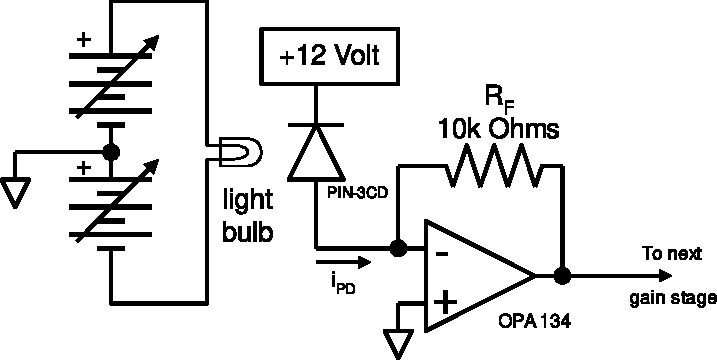
\includegraphics[width=0.5\textwidth]{figures/tamp_schematic.pdf}
    \caption{
        Current measurement across a photo diode using a transimpedance amplifier setup. Assuming no current flows into the amplifier input, the current through $R_f$ has to be exactly the current $I + I_0$ flowing through the diode. This allows for very precise measurement of $\langle I^2 \rangle$.
        Provided by \autocite{instructions}.
    }
    \label{fig:transimpedance schematic}
\end{figure}
Charge is transported through a conductor only in multiples of the elementary charge $e$. This produces a type of noise called \textit{Shot Noise} which becomes relevant for very small currents. The variance of the noise current across an electric component is
\begin{equation}
    \label{eq:shot noise}
    S_I\;\Delta f = \langle I^2 \rangle = 2 e\; I_0\; \Delta f + S_0\;\Delta f
\end{equation}
as shown in \autocite{Buch}. Note that the total current is $I_0 + I$ with the mean noise current $\langle I \rangle = 0$. Again, an additional noise source $S_0$ was added, accounting for the signal processing chain. According to \autoref{eq:shot noise} the value of $e$ can be calculated if $I_0$ is known, because the additional component $S_0$ can be eliminated by measuring the same component at different currents, and computing the derivative
\begin{equation}
 e = \frac{1}{2}\frac{\Delta S_I}{\Delta I_0}
\end{equation}

The current can be measured in two different ways: 
It can be determined by connecting a resistor in series with the diode and measuring the voltage drop across it, similar to how Johnson noise was measured in the previous part. 
Another way is to use an amplifier which produces an output voltage proportional to an input current, a so-called \textit{transimpedance amplifier}.The schematic using the latter setup is shown in \autoref{fig:transimpedance schematic}. A lamp with variable brightness next to the photo diode allowed for adjustment of the mean current $I_0$.

\begin{figure}[h!]
    \centering
    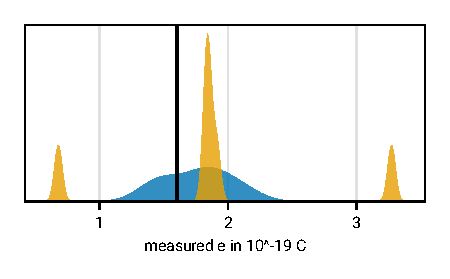
\includegraphics{figures/03 shot noise.pdf}
    \caption{
        Distribution of the measured value for $e$, by measuring the voltage over a resistor (blue), using a trans-impedance amplifier (yellow).
        Corrected measurements, assuming different gain setting (green). 
        The literature value is marked by the black line.
    }
    \label{fig:shot noise}
\end{figure}
% The estimated values for $e$ using the two methods respectively are $\SI{1.76(25)e-19}{C}$ and $\SI{1.9(08)e-19}{C}$, which are both in agreement with the literature value of $\SI{1.602e-19}{C}$.
% \textbf{Discuss the corrections for the wrong data point.}

As there is no structure in the measured values for $e$ over bandwidth or current, the distribution of the measured values is shown in \autoref{fig:shot noise}.
Here the measurements over the resistors have a mean value of $\SI{1.76(25)e-19}{C}$, with a statistical uncertainty.
This is compatible with the literature value of $\SI{1.602e-19}{C}$.\\
The measurement using the transimpedance amplifier shows two outliers in the histogram, coincidentally at about $2 \cdot e$ and $e/2$.
They are caused by the same, likely incorrect data point. During one measurement the noise is suspiciously large. The result is an inflated, computed value for $e$ from the discrete derivative between the previous data point and the one in question, and a deflated value for the following one. The gain setting on the output amplifier was likely read off incorrectly. 
Assuming the setting next too it, the measurement can be corrected, yielding a value of \SI{1.897(68)e-10}{C}.
This demonstrates the advantage of using the lower noise transimpedance amplifier configuration.

Our results are consistently too large, implying a additional with $I_0$ correlated noise source. 
This could be the power supply for the lamp.

\section{Discussion}
In the grand scheme, our measurements show that both types of noise behave mostly as expected. Looking in detail however, they deviate significantly from theory in several aspects, most notably in case of Johnson-Noise with respect to temperature.

\section{Conclusion}
The experiment setup \textbf{NF1-A} by \textit{TeachSpin, Inc.} provides good results while generating little additional noise in the signal processing chain. This allows for quantitative measurements of Johnson-Nyquist noise and shot noise to determine the Boltzmann constant and the elementary charge. The obtained results are close to literature values, but differ significantly due to consistent, additional noise sources which could not be located conclusively. Only the temperature-dependent yielded questionable result, subject to a strange type of noise varying with resistance and most curiously, temperature. Unfortunately, the available measurement data does not allow for further investigation. Quantifying the results is therefore difficult, and the determined temperature value at absolute zero is significantly lower than expected.

\addcontentsline{toc}{section}{Literature}
\nocite{*}
\printbibliography

\end{document}
